\documentclass[11pt,a4paper]{article}
\usepackage[utf8]{inputenc}
\usepackage[T1]{fontenc}
\usepackage{lmodern}
\usepackage[a4paper,margin=2.4cm]{geometry}
\usepackage{setspace,microtype,graphicx,booktabs,tabularx,longtable,array,enumitem,hyperref,xcolor,float,caption}
\usepackage{tikz}
\usepackage[backend=biber,style=authoryear,sorting=nyt,maxcitenames=2,maxbibnames=99]{biblatex}
\usepackage{xurl}
\addbibresource{references.bib}
\usetikzlibrary{arrows.meta,positioning,shapes.geometric,calc}
\hypersetup{colorlinks=true,linkcolor=blue!50!black,citecolor=blue!50!black,urlcolor=blue!60!black,pdftitle={Responsible AI Technical Report: BrainWaveNet},pdfauthor={Levi Pedro Tejedor Rico}}
\setstretch{1.12}
\setlength{\parskip}{0.5\baselineskip}
\captionsetup{font=small,labelfont=small,textfont=small}
\setlist[itemize]{leftmargin=*,itemsep=2pt,topsep=2pt}
\setlist[enumerate]{leftmargin=*,itemsep=2pt,topsep=2pt}
\newcolumntype{Y}{>{\raggedright\arraybackslash}X}
\newcommand{\ASD}{\textsc{asd}}
\newcommand{\TD}{\textsc{td}}
\newcommand{\PBG}{\textsc{pbg}}
\newcommand{\SUM}{\textsc{sum}}
\newcommand{\FAST}{\textsc{fast}}

\title{\textbf{Technical Report: Responsible AI Assessment of BrainWaveNet}\\
\large Responsible AI Assessment for Autism Spectrum Disorder Research}
\author{Levi Pedro Tejedor Rico\\Student ID: 4506001}
\date{Module: CSI\_7\_DEL -- Deep Learning}

\begin{document}
\maketitle

\begin{abstract}
This report assesses BrainWaveNet, a wavelet-based Transformer that classifies autism spectrum disorder (ASD) and typically developing participants using resting-state functional MRI. It combines Leslie's SUM values (Respect, Connect, Protect and Care), FAST principles (Fairness, Accountability, Sustainability and Transparency), and process-based governance across the AI lifecycle. BrainWaveNet is a research prototype evaluated on ABIDE-I; its reported performance and lack of external clinical validation do not support diagnostic use. The assessment identifies evidence gaps in stakeholder participation, subgroup evaluation, test-set governance, reproducibility and operational oversight. It proposes proportionate governance gates, accountable roles and social impact assessment checkpoints. The recommendation is to restrict the model to research until independent validation, meaningful autistic community participation and appropriate clinical safety governance have been demonstrated. It identifies evidence requirements for reproducibility, human oversight and post-release review if clinical evaluation is proposed. Documented facts are distinguished from recommendations, and remaining limitations are recorded for future work.
\end{abstract}

\tableofcontents
\newpage

\section{Introduction}
This report evaluates whether BrainWaveNet is suitable for use in a human healthcare environment and examines what would be required for its responsible redevelopment. The project is a deep-learning research model that analyses resting-state functional magnetic resonance imaging (rs-fMRI) data to classify participants into an ASD group or a typically developing control group. The ethical question goes beyond technical classification: whether the model's purpose, evidence base, design choices and governance justify any real-world use that could affect autistic people must also be considered. In particular, its binary ASD/control target may simplify a heterogeneous condition and should not be mistaken for a complete account of individual characteristics or support needs.

To answer this, the evaluation applies Leslie's SUM values alongside the FAST principles, translating them directly into a process-based governance (PBG) framework spanning problem formulation, data acquisition, preprocessing, modelling, validation, and deployment. The report distinguishes between information explicitly documented in the published research and issues for which evidence is not available. The absence of information in a paper is treated as an evidence gap, not as proof of deliberate omission. Recommendations are therefore based on the evidence that is currently available.

The scope encompasses this specific model, dataset, and public code implementation, paying close attention to social impact, fairness, accountability, transparency, sustainability, privacy, clinical safety, and technical validity. The analysis relies strictly on the BrainWaveNet paper, ABIDE-I documentation, and the linked public repository; experiments are not independently re-run and identifiable participant data are not handled.

Naturally, this document is neither a clinical trial report, a formal legal opinion, nor a certified medical-device conformity assessment. The assessment does not infer individual diagnostic capacity from group-level statistics or assume that the permissions governing a public research dataset automatically extend to new clinical applications. Where sources omit governance workflows, an evidence gap is recorded and safeguards are proposed rather than misconduct being assumed. Section 2 outlines the clinical and technical context, Section 3 maps out the SUM/FAST assessment alongside lifecycle controls and decision gates, and Section 4 concludes with concrete recommendations for deployment.

\section{AI Project Background}
\subsection{Clinical and research context}
Autism spectrum disorder (ASD) is a heterogeneous neurodevelopmental condition. Clinical understanding involves developmental history, behaviour and the individual's own experiences; neuroimaging research explores whether group-level patterns of brain activity and functional connectivity may contribute to scientific understanding. Resting-state functional magnetic resonance imaging (rs-fMRI) measures blood-oxygen-level-dependent signals while a participant is not performing a specified task. Researchers use these signals to study functional relationships between brain regions. Such measurements are research signals rather than direct measures of a person's identity, abilities or support needs.

The Autism Brain Imaging Data Exchange (ABIDE) was established as a multi-site research resource to facilitate investigation of autism using neuroimaging and phenotypic information. ABIDE-I brings together imaging and participant information collected by different research sites, enabling researchers to study patterns across datasets that would be difficult for a single centre to assemble (\cite{dimartino2014,abidewebsite}). Its multi-site character is scientifically valuable, while making harmonisation and generalisability important considerations for studies using the resource.

\subsection{BrainWaveNet as a research approach}
Jeong et al. (2024) introduce BrainWaveNet, a deep-learning approach that combines wavelet analysis with a Transformer architecture to classify rs-fMRI patterns in ASD research. The method applies a complex Morlet continuous wavelet transform to blood-oxygen-level-dependent (BOLD) time series, then uses residual convolutional blocks and temporal and spatial attention modules to learn frequency-domain and spatiotemporal representations. The approach is designed to capture information at different temporal frequencies while modelling relationships across brain regions.

The published pipeline uses CPAC-preprocessed imaging, a 0.01--0.1 Hz band-pass filter, no global signal regression and the Craddock 200 atlas. The authors describe cropping time series to a common length and representing signals through five frequency sub-bands. These are methodological choices reported in the paper, not independently validated choices in this coursework (\cite{jeong2024}).

BrainWaveNet should be understood as a research classifier developed to distinguish labelled groups in a retrospective neuroimaging dataset. Its architecture and reported experimental results are part of the prior research literature; they do not, by themselves, establish a clinical diagnostic role, individual-level validity or benefit to patients. The distinction between research classification and clinical diagnosis is central to interpreting the project and is examined in the assessment that follows.

\subsection{From imaging signal to computational representation}
An rs-fMRI scan produces a sequence of volumetric images rather than a direct readout of neural activity. Preprocessing typically addresses motion and other acquisition artefacts, aligns images, and maps regional signals into a common representation. An atlas divides the brain into regions of interest; correlations or other temporal features can then be used to describe functional connectivity. Each stage introduces assumptions: motion correction cannot remove every artefact, atlas choice changes regional boundaries, and filtering determines which temporal variation is retained. Results therefore depend on acquisition and processing choices as well as the learning algorithm.

\section{Responsible AI Assessment}

\subsection{Project-specific evidence and data audit}
Jeong et al. report 897 participants after quality-control exclusions (414 ASD; 483 controls), a 7:2:1 split and five-fold cross-validation. Reported mean performance was AUC 0.7388, accuracy 67.55\%, sensitivity 66.49\% and specificity 68.35\%. These are retrospective paper results, not independently reproduced here; external clinical validation is not reported (\cite{jeong2024}).

The released ABIDE-I phenotype file audited for this project contains 1,112 records (539 ASD; 573 controls), including 948 males and 164 females. The ASD group contains 474 males and 65 females; controls contain 474 males and 99 females. It has 20 SITE\_ID labels. Di Martino et al. report the same total but different diagnostic counts (533 ASD; 579 controls), and state that 25\% of sites excluded females by design (\cite{dimartino2014}). The discrepancy is retained rather than reconciled without evidence.

Six quality-control fields are missing for 13 participants (10 ASD; 3 controls). Among complete cases, mean functional mean framewise displacement is 0.1619 for ASD (n=529) and 0.1026 for controls (n=570). These descriptive figures refer to the 1,112-record phenotype file, not the 897-person BrainWaveNet cohort. They identify representativeness and data-quality questions; they do not establish model bias or explain its predictions.

\begin{figure}[H]
\centering
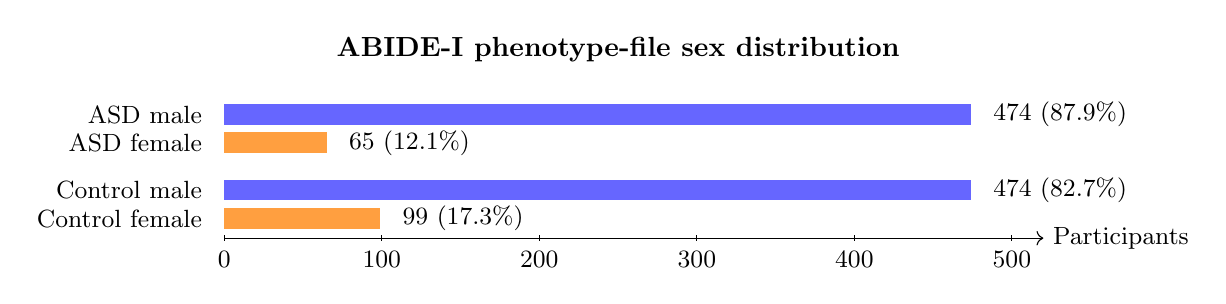
\begin{tikzpicture}[x=0.020cm,y=0.48cm,font=\small]
\node[font=\bfseries] at (250,5.0) {ABIDE-I phenotype-file sex distribution};
\draw[->] (0,0) -- (520,0) node[right] {Participants};
\foreach \x in {0,100,200,300,400,500} {\draw (\x,0.08) -- (\x,-0.08) node[below] {\x};}
\fill[blue!60] (0,3.0) rectangle (474,3.55);
\fill[orange!75] (0,2.25) rectangle (65,2.80);
\fill[blue!60] (0,1.0) rectangle (474,1.55);
\fill[orange!75] (0,0.25) rectangle (99,0.80);
\node[anchor=east] at (-8,3.27) {ASD male};
\node[anchor=west] at (482,3.27) {474 (87.9\%)};
\node[anchor=east] at (-8,2.52) {ASD female};
\node[anchor=west] at (73,2.52) {65 (12.1\%)};
\node[anchor=east] at (-8,1.27) {Control male};
\node[anchor=west] at (482,1.27) {474 (82.7\%)};
\node[anchor=east] at (-8,0.52) {Control female};
\node[anchor=west] at (107,0.52) {99 (17.3\%)};
\end{tikzpicture}
\caption{Sex counts in the audited ABIDE-I phenotype file (539 ASD; 573 controls). These are not the sex breakdown of BrainWaveNet's 897-participant analysis cohort. The source records binary male/female categories and does not report model performance by sex.}
\label{fig:abide-sex}
\end{figure}

\begin{figure}[H]
\centering
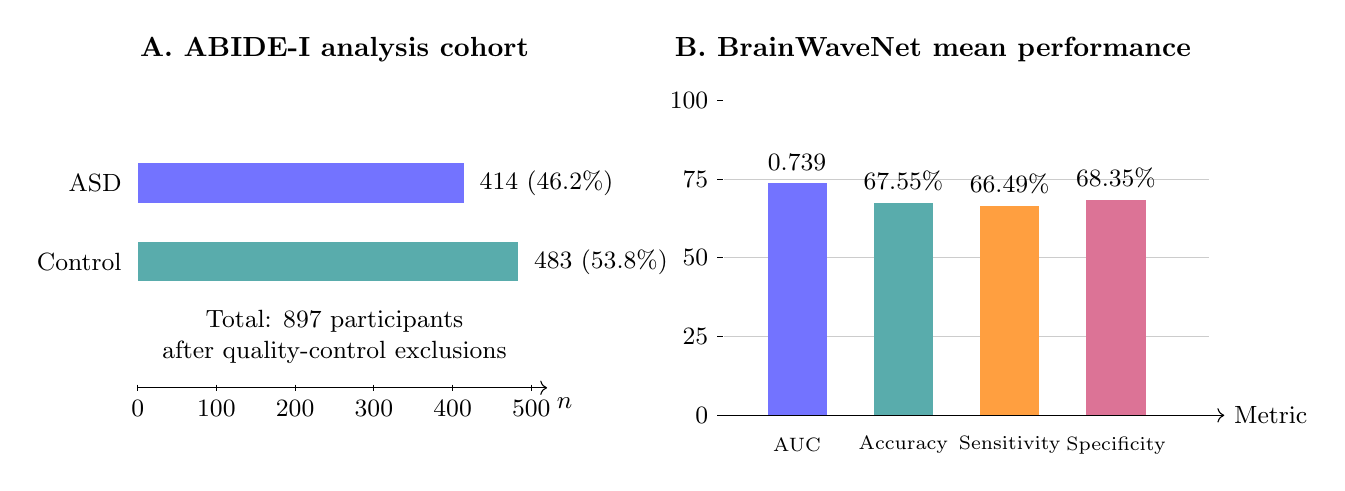
\begin{tikzpicture}[font=\small]
% Panel A: cohort composition
\node[font=\bfseries] at (2.5,3.5) {A. ABIDE-I analysis cohort};
\begin{scope}[yshift=-0.8cm]
\draw[->] (0,0) -- (5.2,0) node[below right] {$n$};
\foreach \x/\lab in {0/0,1/100,2/200,3/300,4/400,5/500} {
  \draw (\x,0.04) -- (\x,-0.04) node[below] {\lab};
}
\fill[blue!55] (0,2.35) rectangle (4.14,2.85);
\node[anchor=east] at (-0.08,2.6) {ASD};
\node[anchor=west] at (4.22,2.6) {414 (46.2\%)};
\fill[teal!65] (0,1.35) rectangle (4.83,1.85);
\node[anchor=east] at (-0.08,1.6) {Control};
\node[anchor=west] at (4.91,1.6) {483 (53.8\%)};
\node[align=center] at (2.5,0.65) {Total: 897 participants\\after quality-control exclusions};
% Panel B: reported performance
\end{scope}
\node[font=\bfseries] at (10.1,3.5) {B. BrainWaveNet mean performance};
\begin{scope}[yshift=-1.15cm]
\draw[->] (7.4,0) -- (13.8,0) node[right] {Metric};
\foreach \y/\lab in {0/0,1/25,2/50,3/75,4/100} {
  \draw (7.36,\y) -- (7.44,\y) node[left=2pt] {\lab};
}
\draw[gray!40] (7.45,1) -- (13.6,1);
\draw[gray!40] (7.45,2) -- (13.6,2);
\draw[gray!40] (7.45,3) -- (13.6,3);
\fill[blue!55] (8.0,0) rectangle (8.75,2.955);
\fill[teal!65] (9.35,0) rectangle (10.10,2.702);
\fill[orange!75] (10.70,0) rectangle (11.45,2.660);
\fill[purple!55] (12.05,0) rectangle (12.80,2.734);
\node[align=center,font=\scriptsize] at (8.375,-0.38) {AUC};
\node[align=center,font=\scriptsize] at (9.725,-0.38) {Accuracy};
\node[align=center,font=\scriptsize] at (11.075,-0.38) {Sensitivity};
\node[align=center,font=\scriptsize] at (12.425,-0.38) {Specificity};
\node[above] at (8.375,2.98) {0.739};
\node[above] at (9.725,2.73) {67.55\%};
\node[above] at (11.075,2.69) {66.49\%};
\node[above] at (12.425,2.76) {68.35\%};
\end{scope}
\end{tikzpicture}
\caption{ABIDE-I cohort composition after the exclusions reported by Jeong et al. (2024), alongside BrainWaveNet's published mean metrics. Cohort percentages are calculated from 414 ASD and 483 control participants. Performance values are reproduced from the paper and were not independently generated in this project.}
\label{fig:abide-performance}
\end{figure}

The paper and README differ on some comparator metrics and the reported accuracy standard deviation. Training code logs test metrics each epoch, although checkpoint selection is described as validation-AUC-based. This creates a risk of test-set feedback, not proof of leakage. The final test set should remain inaccessible until development decisions are frozen. Attention-based region rankings are exploratory, not causal explanations or validated biomarkers.

\subsection{SUM values}
Leslie's SUM values—Respect, Connect, Protect and Care—translate ethical aims into project requirements (\cite{leslie2019}).

\begin{table}[H]
\centering
\small
\begin{tabularx}{\textwidth}{p{1.8cm}Y Y}
\toprule
\textbf{Value} & \textbf{Assessment} & \textbf{Required response} \\
\midrule
Respect & ABIDE reports local ethics review or waiver and anonymisation. Consent scope and all secondary-use conditions are not established by the reviewed sources. & Verify consent and data-use permissions; restrict access and re-identification risks. \\
Connect & Autistic participation in BrainWaveNet decisions is not documented; this is an evidence gap, not proof of no consultation. & Involve autistic people in priorities, proposed-use reviews and accessible communication; compensate participation. \\
Protect & The audited file is 85.3\% male; the retained model cohort has no reported sex breakdown. Motion also differs between diagnostic groups. & Report recruitment, exclusions and subgroup errors; avoid population-wide claims. \\
Care & Retrospective classification does not demonstrate improved wellbeing. Misclassification may cause distress, stigma or inappropriate decisions. & Maintain research-only use; never determine diagnosis or access to support (\cite{topol2019,who2021}). \\
\bottomrule
\end{tabularx}
\caption{Assessment of BrainWaveNet against SUM values.}
\label{tab:sum}
\end{table}

A secure classifier may still be harmful if a group-level research output is treated as an individual diagnosis. Ethical acceptability therefore depends on purpose, participation and consequences, not data protection alone.

\subsection{FAST principles}
FAST makes ethical aims operational. Fairness concerns distribution of benefits and errors; Accountability assigns responsibility; Sustainability considers long-term impacts; Transparency makes purpose and limits understandable (\cite{leslie2019}).

\begin{table}[H]
\centering
\small
\begin{tabularx}{\textwidth}{p{1.8cm}Y Y}
\toprule
\textbf{Principle} & \textbf{Risk or evidence gap} & \textbf{Control} \\
\midrule
Fairness & Aggregate metrics only; no age, sex, site or clinical subgroup results. The phenotype audit is male-skewed and shows higher mean motion in ASD. These are representativeness and confounding concerns, not proof of bias (\cite{jeong2024,dimartino2014}). & Justify the target; report subgroup errors, calibration and uncertainty; test motion and site sensitivity (\cite{abraham2017,mehrabi2021,suresh2021,rajkomar2018,obermeyer2019}). \\
Accountability & No clinical owner, release authority or incident process is identified. Test metrics are logged during training. & Name human owners; freeze test access; log decisions; define approval, pause and withdrawal authority (\cite{raji2020,who2021,gmlp2021}). \\
Sustainability & Energy, hardware, maintenance and long-term costs are unreported. & Assess computational and institutional capacity and community impacts at each SIA review (\cite{leslie2019,who2021}). \\
Transparency & The paper--README metric differences remain unresolved; accessible explanations for affected people are not established. & Reconcile results; version the pipeline; publish a model card covering purpose, uncertainty, intended use and limits (\cite{mitchell2019,who2021,gmlp2021}). \\
\bottomrule
\end{tabularx}
\caption{Assessment against FAST principles.}
\label{tab:fast}
\end{table}

The binary ASD/control target cannot represent the diversity of autistic characteristics and support needs. Any future research into specific characteristics would require validated measures and professional interpretation. Fairness reporting must also protect small groups; validation and monitoring require resources. These trade-offs belong in the risk register.

\subsection{PBG landscape, roles and decision gates}
The proposed process-based governance (PBG) framework spans five lifecycle phases. The sponsor owns purpose and resources; the ML/data lead maintains technical records; the data steward documents provenance; the privacy specialist reviews access; an independent reviewer challenges validation; the clinical safety lead owns the safety case; autistic representatives contribute to decisions; and a release board records approvals and residual risks.

\small
\setlength{\LTcapwidth}{\textwidth}
\setlength{\tabcolsep}{3pt}
\begin{longtable}{>{\raggedright\arraybackslash}p{2.2cm} >{\raggedright\arraybackslash}p{6.68cm} >{\raggedright\arraybackslash}p{6.68cm}}
\caption{Lifecycle ethical examination and proposed PBG controls. Evidence gaps are not treated as proof of misconduct; controls are recommendations, not completed actions.}
\label{tab:lifecycle}\\
\toprule
\textbf{Phase} & \textbf{Ethical examination} & \textbf{PBG control and gate} \\
\midrule
\endfirsthead
\toprule
\textbf{Phase} & \textbf{Ethical examination} & \textbf{PBG control and gate} \\
\midrule
\endhead
\midrule
\multicolumn{3}{r}{\small\itshape Continued on next page}\\
\endfoot
\bottomrule
\endlastfoot
Problem formulation & Binary classification is not a demonstrated patient benefit or diagnostic pathway. Autistic co-design is not documented. & Sponsor and autistic advisers define purpose, stakeholders, alternatives and prohibited uses. Complete Alpha SIA before data use; stop if purpose and participation are unjustified.\\
Data acquisition & The phenotype file is male-skewed and has 13 records with incomplete QC fields. Consent scope and secondary-use conditions need confirmation. & Data steward records provenance, permissions, consent basis, demographics, missingness and quality. Privacy lead reviews access, retention and re-identification risk.\\
Preprocessing & CPAC, filtering, parcellation, cropping and wavelet transformation are paper-reported but not independently reproduced here. Exclusions may affect group representation. & Version code, parameters and environment; log exclusions; test motion thresholds and site effects. Review at Alpha-to-Beta.\\
Modelling and validation & Internal metrics are reported, but subgroup and independent external clinical validation are not. Test logging creates exposure risk; random splits alone do not establish site generalisation. & Independent reviewer freezes participant-level test data and assesses subgroup errors, calibration, uncertainty and site-held-out/external performance. No progression without acceptable evidence and a model card.\\
Deployment and monitoring & No clinical deployment, prospective monitoring, incident process or safety case is evidenced. Repository availability is not clinical authorisation. & Retain research-only restriction. Any future pilot needs approvals, trained users, human review, complaint routes, drift/subgroup monitoring, pause and rollback thresholds, and SIA reassessment.\\
\end{longtable}
\normalsize

\begin{figure}[H]
\centering
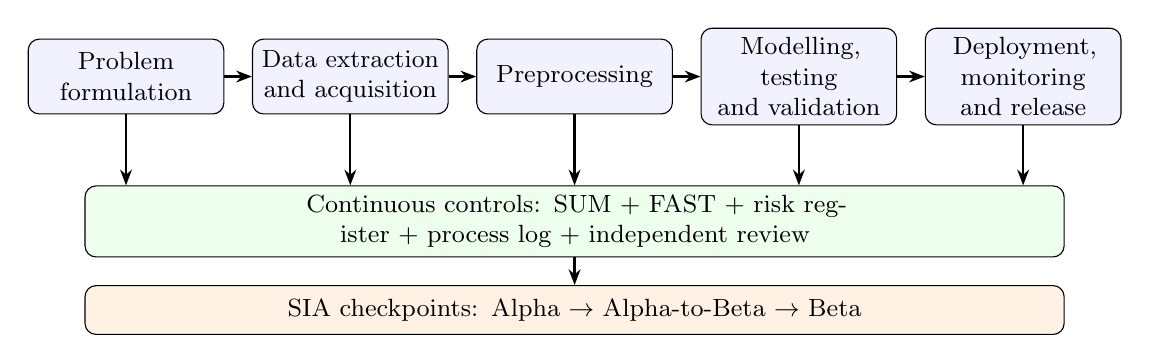
\begin{tikzpicture}[
    node distance=0.35cm,
    stage/.style={draw,rounded corners,align=center,text width=2.25cm,minimum height=0.95cm,font=\small,fill=blue!5},
    gate/.style={-{Stealth[length=2mm]},thick},
    band/.style={draw,rounded corners,align=center,fill=green!7,text width=12.2cm,minimum height=0.62cm,font=\small}
]
\node[stage] (p) {Problem\\ formulation};
\node[stage,right=of p] (d) {Data extraction\\ and acquisition};
\node[stage,right=of d] (x) {Preprocessing};
\node[stage,right=of x] (m) {Modelling, testing\\ and validation};
\node[stage,right=of m] (r) {Deployment, monitoring\\ and release};
\draw[gate] (p) -- (d);
\draw[gate] (d) -- (x);
\draw[gate] (x) -- (m);
\draw[gate] (m) -- (r);
\node[band,below=0.9cm of x] (sf) {Continuous controls: SUM + FAST + risk register + process log + independent review};
\node[band,below=0.35cm of sf,fill=orange!10] (sia) {SIA checkpoints: Alpha $\rightarrow$ Alpha-to-Beta $\rightarrow$ Beta};
\draw[gate] (p.south) -- (p.south |- sf.north);
\draw[gate] (d.south) -- (d.south |- sf.north);
\draw[gate] (x.south) -- (x.south |- sf.north);
\draw[gate] (m.south) -- (m.south |- sf.north);
\draw[gate] (r.south) -- (r.south |- sf.north);
\draw[gate] (sf) -- (sia);
\end{tikzpicture}
\caption{Proposed PBG structure. Ethical review is continuous, with SIA checkpoints at lifecycle transitions.}
\label{fig:pbg}
\end{figure}

The process log should retain dataset permissions and versions, preprocessing and exclusions, code/model versions, split identifiers, validation and fairness results, risk decisions, approvals and incidents. Participant-level records require access controls; accountable humans—not the model—own decisions.

At Alpha, assess purpose, alternatives, affected groups and impacts before data use. At Alpha-to-Beta, resolve critical risks and document stakeholder review and release-board decisions. Beta reassessment applies only after a future authorised implementation: monitor harms and drift, investigate complaints, and pause or withdraw when thresholds are breached. Owners and review dates must be set before any pilot. These checkpoints follow Leslie's SIA and PBG guidance (\cite{leslie2019}).

\section{Conclusion}
BrainWaveNet remains a research prototype: its ABIDE-I results do not justify diagnosis or autonomous decisions. The phenotype audit identifies sample imbalance and diagnosis-associated motion differences, but is descriptive and does not evaluate model predictions. The reviewed evidence does not establish autistic co-design, subgroup performance, external clinical validation, full reproducibility or operational monitoring. These are evidence gaps, not proof of harm. The binary target also cannot represent individual autistic people's varied characteristics and support needs; any future validated measures would require professional interpretation and must not replace the person's voice.

The model should remain research-only under the proposed PBG framework. Complete the initial SIA at Alpha and review it at Alpha-to-Beta. Beta reassessment is conditional on future authorised implementation. Clinical use must remain prohibited unless patient-relevant need, stakeholder support, independent validation, safety evidence, approvals and human oversight are demonstrated.

Immediate work should protect the final test set, reconcile paper--repository discrepancies, version the development pipeline, publish a model card and assign accountable owners. Any future pilot must be limited, supervised and reversible, with monitoring for drift, errors, complaints and unintended impacts. Outputs must be identified as research classifications, not diagnoses, and must not determine access to support. If these conditions cannot be met, the responsible decision is not to deploy BrainWaveNet.

\printbibliography[heading=bibintoc,title={References}]

\end{document}
